\section{Content Selection Models for Streaming Summarization}

We propose two novel approaches to the streaming summarization task
using biased affinity propagation (AP) clustering \citep{frey2007clustering}
and learning-to-search (L2S) \citep{daume2009search,chang2015learning}.
These models led to the publication of two papers 
\citep{kedzie2015predicting,kedzie2016real}, in addition to participation 
in the TREC Temporal Summarization tracks where we were the top performer in
2014 and the fourth and fifth place performer in 2015 \citep{aslam2015trec,aslam2016trec}. 

In the Temporal Summarization track, the grounding scenario was disaster
summarization, where a participant system received a brief query string 
$\query$ describing a natural or man-made disaster, and the system was 
expected to process a time-ordered stream of documents relevant to the query, 
extracting sentences that were likely to contain important facts about the
event. Each query corresponded to a real-life disaster that was significant
enough to have an associated entry in Wikipedia.

For each query, human annotators also collected a reference set of important 
facts, which we refer to as \textit{nuggets}, 
from the revision history of that query's associated Wikipedia page. 
Nuggets consist of a piece of reference text and timestamp for when this piece
of information first appeared in the Wikipedia revision history. 
See \autoref{fig:eventsnuggets} for example queries and nuggets.

\input{3_fig_events_and_nuggets.tex}

We will refer to the set of extracted sentences as the update or extract
summary interchangeably. Similarly, we will use the phrases extract a sentence,
select a sentence, or emit a sentence to mean we add a sentence in the 
document stream to our rolling update summary. If a sentence $\strsent$ 
expresses the same piece of information as a nugget text $\nugget$ 
we say that $\strsent$ contains $\nugget$ or $\nugget \in \strsent$.

Systems are rewarded when they find sentences that contain important and novel
nuggets. Systems are penalized for 
selecting sentences that are irrelevant (i.e. contain no nuggets) or 
contain nuggets already covered by previous updates. 
Latency penalized metrics are also computed where
the importance of a nugget decays over time. E.g. if a system
recovers the nugget ``25 people were reported injured,'' several days
after this fact was first reported, it will receive less credit for it
than the system that emits that nugget an hour after it enters the 
document stream. See \cite{aslam2014trec} for more details on this decay 
factor. Intuitively, latency penalized metrics capture the idea that stale
information in a rapidly evolving disaster is less useful and possibly
distracting.

Streaming summarization is a very hard task compared to single and 
multi-document summarization. In the latter case, the context for the 
summarization is fixed, and the input documents are usually quite 
topically focused, minimizing the prevalence of completely irrelevant 
information. In fact, in most multi-document evaluation settings, the
document collections were manually created leading to very topically
coherent text collections. 
\cite{baumel2016topic} for example found that the DUC
query focused summarization datasets are so on topic that a summarization
system could completely ignore the query and perform just as well as a
query aware system.

\begin{figure}
\begin{subfigure}{.47\textwidth}
\begin{algorithmic}[1] 
\Procedure{OracleSummarize}{}
  \State $\updates \gets \varnothing$ \Comment{Init. update summary.}
  \State $\hat{\nuggets} \gets \varnothing$ \Comment{Init. found nuggets.}
  \For{$\strsent \in \strsents$} 
    \If{$\exists \nugget$ s.t. $\nugget \in \strsent
            \wedge \nugget \notin \hat{\nuggets}$ }
      \State $\mathcal{U} \gets \mathcal{U} \cup \{\strsent\}$ 
      \State $\hat{\mathcal{N}} \gets \hat{\mathcal{N}} \cup \{\nugget \in \strsent\}$ 
    \EndIf
  \EndFor
  \State \Return $\mathcal{U}$
\EndProcedure
\end{algorithmic}
    \caption{Greedy oracle streaming summarization algorithm.}
    \label{alg:ts_greedy_oracle}
\end{subfigure}
~
\begin{subfigure}{.48\textwidth}
\begin{algorithmic}[1] 

  \Procedure{GenericSummarize}{}
  \State $\mathcal{U} \gets \varnothing$ \Comment{Init. update summary.}
  \For{$\strsent \in \mathcal{S}$} 
    \State $\hat{\salience} \gets \operatorname{salience}(\strsent, \query) $
    \State $\similarity \gets \operatorname{similarity}(\strsent, \updates)$
    \State $\extract \gets \operatorname{decide}(\hat{\salience}, \similarity)$
    \If{$\extract = 1$}
        \State $\updates \gets \updates \cup \{\strsent\}$
    \EndIf
  \EndFor
  \State \Return $\updates$
\EndProcedure
\end{algorithmic}
    \caption{Greedy generic streaming summarization algorithm.}
    \label{alg:ts_greedy_generic}
\end{subfigure}
\caption{Oracle and generic greedy stream summarization algorithms. 
$\mathcal{S}$ is a time-ordered set of sentences from the document stream 
for query $\query$.}
\end{figure}



%?When considering whether or not to select a sentence for the update summary
%?there are two considerations. First we must estimate the salience, or 
%?importance, of the sentence with respect to the query. This is a proxy
%?for assesing whether or not a sentence contains a nugget. 
%?Second, we must consider
%?whether the relative importance of the sentence in the context of previous
%?updates and current candidate updates warrants selecting it for the summary.
%?This is a proxy for determining if the sentence contains any novel nuggets
%?with respect to our current update summary.


If we had clairvoyant knowledge of which nuggets were contained in each
sentence in the document stream,
this task would be trivial in that the greedy algorithm in 
\autoref{alg:ts_greedy_oracle} would return an approximately optimal summary.
Since we do not know this information at test time, we attempt approximate
the if-statement in line 5 of the oracle by answering the following proxy 
questions:
\begin{enumerate}
    \item How salient is sentence $\strsent$ with respect to query $\query$?
    \item How similar is the sentence $\strsent$ with respect to the set of 
            previously selected updates $\hat{\strsent} \in \updates$?
\end{enumerate}
The generic stream summarization algorithm we aim to implement is presented
in \autoref{alg:ts_greedy_generic}.

The two models we propose to solve these more tractable problems come with
different trade-offs. They both, however, rely on a feature-base 
representation of the stream sentences to make salience and selection 
predictions. In the next sub-section, we describe the different feature
groups before describing each of the models used to perform the streaming
summarization task.







%In the next sections, we describe to proposed solutions to this problem.
%Both approaches use feature-based regression models to eestimate sentence
%salience and so we briefly describe the features here.

\input{3_fig_features.tex}

\subsection{Features for Sentence Importance Estimation}

The streaming summarization problem is difficult precisely because the context
is constantly shifting. We cannot rely solely on word frequency because
the counts of particular ngrams will be shifting throughout the period of 
interest. Instead we compute several groups of sentence features that are
specifically helpful for the query focused task. We divide our features
into two groups: static and dynamic features. Static features do not take into
account previous sentence selection decisions, while dynamic features
can be used information about current state of the update summary or stream
behaviour. \autoref{fig:strfeats} shows which feature groups were used 
in each of our two approaches. In general, incorporating dynamic features
into the learning-to-search approach is much easier.


\subsubsection{Static Features}
\paragraph{Simple Surface Features} 

The document stream that we will be operating over is incredibly noisy,
full of automatically extracted article text from raw web pages in 
dramatically different formatting. As a result, the underlying text is often
full of wep page headers, headlines to other stories, and irrelevant link text.We this group of basic features to help identify typical content bearing
sentences in the AP news style \citep{ap_style_guide}. These features 
include sentence length, the average number of capitalized words,
document position, sentence length in words, and the average number of 
named entities. Length and position features have been used previously in
other learning based models of sentence salience
\citep{kupiec1995trainable,conroy2001using}.

\paragraph{Query Features} To ensure the focus of the update summaries,
we employ query match features that count frequency of query term matches
in the sentence. We also do a simple query expansion using WordNet 
\citep{miller1995wordnet}
to find  synonyms, hypernyms, and hyponyms for the query event type and compute
a similar term match count with the expansion.
Queries in the Temporal Summarization data are also labeled with even type.
See \autoref{fig:eventtypes} for the list of query event types we used. 
For the \emph{earthquake} query type, for example, we find the following terms:
``quake'', ``temblor'', ``seism'', and ``aftershock''.


\begin{table}
\begin{tabular}{r | l}
\textbf{Event Type} & \textbf{Event Queries} \\
\hline
Storm & hurricane isaac, hurricane sandy, midwest derecho, typhoon bopha\\
Earthquake & guatemala earthquake  \\
Meteor Impact & russia meteor \\
Accident & buenos aires train crash,  pakistan factory fire\\
Riot & egyptian riots\\
Protest & bulgarian protests, egyptian protests \\
Hostages & in amenas hostage crisis \\
Shooting & colorado shooting, sikh temple shooting\\
Bombing & boston marathon bombing, hyderabad explosion \\
Conflict & konna battle \\
\end{tabular}
\caption{TREC Temporal Summarization query event types with example queries.} 
\label{fig:eventtypes}
\end{table}

\paragraph{Language Model Scores}

We rely on a pair of language models to assess the likelihood of observing
a given sentence in the document stream. The first language model is 
intended to be a generic news model, trained on New York Times and 
Associated Press sections of the Gigaword corpus \citep{graff2003english}. 
This model serves a similar purpose as the simple surface features in helping
to identify newswire-like sentences that are likely to contain informative
content.
The second model is query type specific and intended to focus the summarizer
on sentences from the same domain of the query. For each query type, we 
constructed an in-domain corpus of Wikipedia news articles belonging to
categories and pages related to the event type. The corpus is 
semi-automatically constructed: first a set of high-level categories are 
selected and then all pages belonging to those initial categories or
any sub-categories are automatically added. 
For example, the language
model for the event type ``earthquake'' is estimated
from Wikipedia pages under the category Category:Earthquakes.
For the actual summarization system features, we use the average token log
likelihood under each model as a feature.
We use the SRILM toolkit \citep{stolke2002srilm} to implement a 5-gram 
Kneser-Ney model \citep{kneser1995improved} for both the general and type
specific language models. 

\paragraph{Nugget Likelihood}
Using human judgements from 2014 Temporal Summarization we were able to obtain
example sentences that contained many of the nuggets in our corpus. We used
these judgements to train an ngram based classifier to predict a binary 
label $y$ for a sentence, with $y=1$ if it contained any event nugget and
$0$ otherwise. We used the probability of $y=1$ as an additional feature.

\paragraph{Single Document Summarization Features}
We used several unsupervised sentence ranking methods from the single 
document summarization literature to get several sentence rank features.
Inspired be the \textsc{SumBasic} summarizer \citep{nenkova2005impact}, we
compute the average and sum of unigram probability of each sentence using 
sentence's document unigram distribution. Inpsired by \citep{guo2013updating},
for each sentence we compute the average cosine distance to the remaining 
sentences in it's enclosing document. Finally, we compute the document
level centroid rank \citep{radev2000centroid} and LexRank 
\citep{erkan2004lexrank} for each sentence.

\subsubsection{Dynamic Features}
\paragraph{Geographic Relevance} 
The queries in the Temporal Summarization data are all grounded to physical
events in the world and we would like to exploit that. For example, while
there are sadly many reports of bombings or explosions at any given time 
around the world, when summarizing the query ``boston marathon bombing'' 
we are only really interested in news from a relatively proscribed 
geographic area, in this case, Boston, Massachusets. Implementing 
a geographic relevance signal is quite difficult in practice since 
we do not have ground truth location data for each event query, and some
events like hurricanes can be on the move. We opt instead to extract all
location mentions (using a named entity tagger) and get the lattitude
and longitude coordinates
of each mention using the Bing maps API \citep{bingmaps}. Location
mentions within the same hour are clustered, and the cluster centers are 
used as the canonical event locations for the query at that time. 
To get features for each sentence in the stream, we find the location of
the news article it came from and then compute average distance of the 
article to the query event locations.


%?The disasters
%?in our corpus are all phenomena that affect some
%?part of the world. Where possible, we would like
%?to capture a sentence’s proximity to the event, i.e.
%?when a sentence references a location, it should be
%?close to the area of the disaster.
%?There are two challenges to using geographic
%?features. First, we do not know where the event is,
%?and second, most sentences do not contain references
%?to a location. We address the first issue by
%?extracting all locations from documents relevant to
%?the event at the current hour and looking up their
%?latitude and longitude using a publicly available
%?geo-location service. Since the documents that are
%?at least somewhat relevant to the event, we assume
%?in aggregate the locations should give us a rough
%?area of interest. The locations are clustered and
%?we treat the resulting cluster centers as the event
%?locations for the current time.
%?The second issue arises from the fact that the
%?majority of sentences in our data do not contain
%?explicit references to locations, i.e. a sequence of
%?tokens tagged as location named entities. Our intuition
%?is that geographic relevance is important in
%?the disaster domain, and we would like to take ad


\paragraph{Temporal Relevance} As we track a query over time, the document
stream will ebb and flow as the underlying event unfolds. With hurricanes
for example, forecasters are usually watching a tropical storm as it grows
and predicitng where it might make landfall. As a result, news about a major
hurricane grows gradually, peaking after its main contact with land
and gradually diminishing. An eartquake on the otherhand gives no warning,
and there is a sudden spike in the query relevant document stream.
While we do not
do an extensive study of different event type shapes (which would certainly 
be very interesting), we would like to take advantage of spiking or bursty
activity in the docuemnt stream as a signal for our summarization system.
We do this by maintaining IDF values for each hour of the document stream.
We create 24 average TF-IDF features for each sentence as if it had occurred
in each of the previous 24 hours; large changes in any of the individual
features should be representative of a spike in the news.

\paragraph{Document Frequency} We also compute the hour-to-hour
percent change in document frequency of the stream. This
feature helps gauge breaking developments in an unfolding
event. As this feature is also heavily affected by the daily
news cycle (larger average document frequencies in the morning
and evening) we compute the 0-mean/unit-variance of this
feature using the training streams to find the mean and variance
for each hour of the day.



\paragraph{Stream Language Models}
We construct several simple unigram language models that we update with 
each new document that we see in the stream. Using these models 
we compute the sum, average, and maximum token likelihood
of the non-stop words
in the sentence. We compute similar quantities restricted to
the person, location, and organization named entities.

\paragraph{Update Similarity} The average and maximum cosine similarity
of the current sentence to all previous updates is computed
under both the tf-idf bag-of-words and latent vector
representation. We also include indicator features for when
the set of updates is empty (i.e. at the beginning of a run) and
when either similarity is 0.


\subsection{Model 1: Salience Biased Affinity Propagation Clustering}

  \begin{figure}
\begin{algorithmic}[1] 
\Procedure{APSalienceSummarize}{}
  \State $\updates \gets \varnothing$ \Comment{Init. update summary.}
  \For{$\strsents_t \in \strsents$} 
    \State $\hat{\Salience} \gets \operatorname{salience}(\strsents_t, \query)$
        \Comment{Estimate sentence salience for each 
                 $\strsent \in \strsents_t$.}
    \State $\Similarity \gets \operatorname{similarity}(
           \strsents_t, \strsents_t)$ \Comment{Compute similarity 
           between each $\strsent_i, \strsent_j \in \strsents_t$.}
    \State $\exemplars \gets \operatorname{AffinityPropagation}(\hat{\Salience}, \Similarity)$ \Comment{Get exemplar sentences $\exemplars$ with AP.}

    \For{$\strsent \in \exemplars$}
      \If{$\hat{\Salience}_\strsent > \lambda_1 \wedge \max \operatorname{similarity}(\updates, \strsent) > \lambda_2$}
        \State $\updates \gets \updates \cup \{\strsent\}$
      \EndIf
    \EndFor
%    \If{$\exists \nugget$ s.t. $\nugget \in \strsent
%            \wedge \nugget \notin \hat{\nuggets}$ }
%      \State $\mathcal{U} \gets \mathcal{U} \cup \{\strsent\}$ 
%      \State $\hat{\mathcal{N}} \gets \hat{\mathcal{N}} \cup \{\nugget \in \strsent\}$ 
%    \EndIf
  \EndFor
  \State \Return $\mathcal{U}$
\EndProcedure
\end{algorithmic}
    \caption{Salience-biased AP clustering based streaming summarization 
             algorithm.}
    \label{alg:ts_sap_algo}
\end{figure}




  Identifying potential updates from the document stream is hard in part
  because we may not have enough context to use word frequencies as a 
  reliable proxy for salience. Our first proposed method accounts for this
  in two ways. 

  First, we process the stream in hourly batches, i.e. we collect all the
  sentences from the last hour and then decide which sentences if any to
  add to the update summary. The trade-off we make is that fast breaking
  events may not immediately be covered by the summarizer.

  Second, we use an exemplar-based clustering algorithm,
  called Affinity Propagation (AP) \citep{frey2007clustering}, that combines
  sentence level salience predictions with pairwise sentence similarities
  to identify a set of exemplar sentences that would make for good 
  additions to the updates summary. The pairwise similarity factors work 
  as our replacement for the ngram-frequency based signal we would normally 
  use in traditional MDS; a sentence that has high overall similarity to
  the other sentences in the batch is likely to be an exemplar and
  more so if it's salience prediction is high relative to the batch.

  Finally, given a set of exemplar sentences $\exemplars$, we add those
  whose maximum similarity to a previous update is below a threshold.
  The final algorithm is presented in \autoref{alg:ts_sap_algo}.



  We describe our process for computing salience and similarity in
 the next sections, before describing the AP clustering algorithm.



%?  We next describe the 
%?
%?
%?
%?  In this model, we process the document stream in hourly batches, 
%?  first predicting the salience of the individual sentences and then 
%?  using affinity propagation (AP) to select a set of exemplar sentences.
%?  Exemplar sentences that have predicted salience above a threshold 
%?  and are below a similarity threshold to previously select sentences are
%?  then emitted to the user as an update summary.





  \subsubsection{Salience Estimation}

  Given a sentence $\strsent \in \strsents$ we would like to predict it's 
  salience with respect to a query $\query$. When we were developing this 
  model,
  we did not have access to many human judgements of query or nugget relevance,
  and so we relied on an automatic measure of sentence salience computable
 from the nugget data we had.

Given a query $\query$, sentence text $\strsent$, and query's nugget texts 
$\nugget \in \mathcal{N}(q)$, we define
the sentence salience $\salience$ as
\[ \salience = \max_{\nugget \in  \nuggets(\query)} \operatorname{similarity}(\strsent, \nugget)\]
where $\operatorname{similarity}(\cdot, \cdot)$ is the cosine similarity of a
low-dimensional representation of the sentence and nugget text.
We used the weighted matrix factorization method of \cite{guo2012simple}
which projects a text's sparse high-dimensional bag-of-words representation
into a dense, low-dimensional vector. We use this method to compute 
sentence similarity in the AP clustering algorithm.


%  Given the feature representation of a sentence, we want to predict how
%confident we are that it contains one or more nuggets. While we have
%many sentences in our corpus, we did not have may sentence level judgements
%about the nuggets that they contained. 
%Lacking these gold annotations, we instead get noisy salience annotations 
%using the maximum similarity of the nugget texts to the sentence texts.
%Formally, given a query $q$, sentence text $s$, and query's nugget texts $n \in \mathcal{N}(q)$
%the sentence salience $y$ is 
%using the following equation:
%\[ y = \max_{n \in  \mathcal{N}(q)} \operatorname{sim}(s, n)\]
%where $\operatorname{sim}$ is a semantic similarity measure (in practice
%we used the weight matrix factorization method of \cite{wmtf}).

We use a Gaussian process-based regression model \citep{rasmussen2004gaussian}
to predict $\salience$ from a feature representation $\phi(\strsent)$ 
\emph{without} knowledge of the nuggets. See \autoref{fig:strfeats}
for the list of feature groups used in the salience regressor.
We use seperate radial basis function (RBF) kernels for each 
feature group, and use the sum of all the kernels as final
kernel matrix for fitting the model.
We fit a separate regressor for each query in our dataset using 1000
randomly sampled sentences from each query's associated relevant document 
stream. At prediction time for a specific query, we hold out that query's salience
model, and use the average prediction of the remaining models to obtain
a salience estimate $\hat{\salience}$ for sentences in the stream.

\subsubsection{Sentence Selection with Salience-biased Affinity Propagation Clustering}


    AP clustering is a factor-graph based clustering
    method that simultaneously selects exemplar data points and maps 
    the remaining data points to one of the exemplars \cite{frey2007clustering}. 
    The exemplar mappings determine the clusters.
    AP has a number of nice properties for extractive summarization.
    First, as an exemplar based clustering method, the cluser center
    is guarantee to be an actual data point observed in the input; 
    this removes the added step of selecting a representative sentence
    if we had used for $k$-means clustering, for example.
    Two, the number of clusters that result is adaptive and 
    based on the interaction of the unary and pairwise factors.

    Given a set of $d$ datapoints $\mathcal{X} = \{x_1, \ldots, x_d\}$, 
    AP finds a set of
    exemplar datapoints $\exemplars \subset \mathcal{X}$ and a mapping
    $A : \mathcal{X} \setminus \exemplars\rightarrow\exemplars$ of the 
    remaining points to one of the exemplars. The configuration of exemplars
    and exemplar assignments is represented as a factor graph, where the
    objective function expresses a net affinity objective:
    
    \[ \mathcal{L}(\mathcal{E}, A) 
        = \exp\left[
            \sum_{i=1}^d \operatorname{affinity}\Big(x_i, A(x_i)\Big) + 
          \log \delta_i \right] \]
    where $\delta_i = \begin{cases} 0 & \textrm{if $A(x_i) \neq x_i$ and $\exists j: j\neq i \wedge A(x_j)=x_i$} \\
1 & \textrm{otherwise}\end{cases}$ is a constraint that enforces all clusters
 have one and only one exemplar and $\operatorname{affinity}:\mathcal{X} 
 \times \mathcal{X} \rightarrow \mathbb{R} $
 is an arbitrary function describing the pairwise similarity of points in 
 $\mathcal{X}$.
 The max-product message passing algorithm,
 a form of loopy belief propagation, can be used to find a configuration
 that approximately maximizes the objective function \citep{dueck2009affinity}.

 We can refactor the first term in the exponent to be 
\[ \sum_{x_i \in \exemplars} \operatorname{affinity}(x_i, x_i) +
 \sum_{x_j \in \mathcal{X} \setminus \exemplars} \operatorname{affinity}(x_j, A(x_j))
 \]
with the first term the sum of unary affinity factors of the exemplars 
and the second term pairwise factors between each non-exemplar datapoint 
and it's exemplar. In the typical case the unary factors are simply 
set to a constant indicating all points are equally likely apriori to serve
as exemplars. In our case, we have some prior beliefs about the importance of 
a given datapoint as expressed by our salience predictions $\hat{\salience}_i$.
Replacing the unary potentials with our salience predictions, 
the pairwise potentials with our semantic similarity function from the 
previous section, and setting $\mathcal{X} = \strsents_t$ 
we arrive at the salience-biased affinity propagation
objective:

 \[ \mathcal{L}(\exemplars, A) = \exp\left[
    \sum_{\substack{\strsent \in \exemplars \\ \hat{\salience} = \operatorname{salience}(\strsent, \query)}} \hat{\salience}  + \sum_{\strsent \in \strsents_t \setminus \exemplars} \operatorname{similarity}\Big(\strsent, A(\strsent)\Big)  + \sum_{i=1}^{|\strsents_t|} \log\delta_i \right].
\] 
When we estimate a sentence to be more salient it is more likely apriori
to form a cluster center. When that sentence is also highly similar to other 
sentences in the batch it collects support from those sentences, further
increasing it's likelihood of being assigned as an exemplar.
 



%~\\
%~\\
%    the net similarity objective
%    \[ \mathcal{L}(X, \mathcal{E}) = 
%    \sum_{i \in \mathcal{E}} \operatorname{salience}(x_i) + \sum_{i \in\mathcal{E}} \sum_{j:e_j = i}\operatorname{similarity}(x_i, x_j)  \]
%    where $\operatorname{salience}$ and $\operatorname{similarity}$ 
%    are unary and pairwise factors that express the degree to which
%    $x_i$ is apriori likey to be an examplar and that $x_i$ is a suitable
%    representative for $x_j$. 
%    $\mathcal{L}$ is optimized using and iterative message passing 
%    algorithm. In the naive setting, $\operatorname{salience}$ is uniform
%    across all $x_i$, i.e. every data point is equally likely to be an
%    exemplar, and exemplar assignment is purely determined by the 
%    pairwise similarity factors.
%    
%    In our present summarization scenario, we have a strong prior belief
%    about suitability of a particular sentence to be an examplar which is
%    represented by the salience predictions $\hat{y}_i$.
% Our system processes hourly batches of sentences 
% $\mathcal{S}_{\textrm{batch}} = \{s_1, s_2, \ldots \}$ by first predicting
% their corresponding saliences $\hat{Y} = \{\hat{y}_1, \hat{y}_2, \ldots\}$.
% We then use AP clustering to find an assignment of exemplar sentences
% that maximizes the following objective:
% \[ \mathcal{L}(\mathcal{S}_{\textrm{batch}}, \mathcal{E}) = 
%    \sum_{i \in \mathcal{E}} \hat{y}_i + \sum_{i \in\mathcal{E}} \sum_{j:e_j = i}\operatorname{similarity}(s_i, s_j)  \]
%    where $\operatorname{similarity}$ is the same WTMF method used in the 
%    noisy salience annotation above. We refer to this method as biased-AP
%    clustering, since the exemplar selection is now biased by our prior
%    beliefs about the sentence's importance to the query.
%
%
%    After the examplars are selected, we perform one final filtering of
%    exemplars, discarding sentences that have a $y_i$ below $\lambda_{sal}$
%    or that have a maximum similarity to any previous updates above
%    $\lambda_{sim}$, where the $\lambda$'s are preset thresholds. 
%    Exemplars that survive filtering are selected for the update summary.

\subsubsection{Data}

  The document stream comes from the news portion of the 2014 TREC
KBA Stream Corpus \citep{frank2012building}, which contains hourly crawls
of the web covering a roughly two year span from 2011 to 2013.
Event queries and their nuggets were taken from the data prepared for 
the 2013 and 2014 TREC Temporal Summarization tracks. This data
contained 25 events and their query strings, period of interest, 
event type. 
Additionally, each event was associated with anywhere from 50 to several
hundred timestamped nugget texts. 
%Each event query was significant 
%enough to have a Wikipedia page. Event nuggets were taken manually
%extracted from the corresponding Wikipedia entry, using the earliest
%revision that contained the nugget to obtain it's timestamp.
For details on the creation of this dataset see \cite{aslam2014trec,aslam2015trec}.
From the larger KBA Stream Corpus we created event specific document 
streams by filtering out any documents that did occur in the period
of interest and contain all the query words of the corresponding event.  



    \subsubsection{Experiments}


Of the 25 events in the TREC TS data, 24 are
covered by the news portion of the TREC KBA
Stream Corpus. From these 24, we set aside
three events to use as a development set. All
system salience and similarity threshold parameters
are tuned on the development set to maximize
\textsc{Rouge-2} \textsc{F1} scores.
We train a salience model for each event using
1000 sentences randomly sampled from the
event's document stream.
We perform a leave-one-out evaluation of each
event. At test time, we predict a sentence’s
salience using the average predictions of the 23
other models.



    Since we lacked gold judgements about what sentences contain which nuggets
    we perform an automatic evaluation using ROUGE \cite{lin2004rouge}. We 
    create reference summaries for each query by concatenating all 
    of it's nugget texts.
    Since there are no fixed summary lengths, and depending on the severity
    of the event, the reference summaries can vary greatly in length.
    To account for this, we report ROUGE recall, precision and F-measure.

    
    We also approximate the manual evaluation of the official TREC TS track
    by automatically mapping sentences to nuggets if their semantic similarity
    is a above a threshold. We report results across a sweep of threshold 
    values from zero to one, with values closer to one a more conservative
    estimate of performance. We report two track metrics: the Expected Gain 
    and Comprehensiveness,  
    which are precision and recall like measures of nugget 
    coverage. If $N$ is the total number of nuggets for a query, $\hat{N}$ is 
    the number of unique nuggets recoverd in our 
    update 
    summary, and $U$ is the total number of sentences extracted for the update
    summary, the Expected Gain and Comprehensiveness are defined as
    \[ \frac{\hat{N}}{U} \quad \textrm{and} \quad \frac{\hat{N}}{N} \]
    respectively. An Expected Gain of 1 would mean that every sentence in
    the update summary contained a novel nugget. Comprehensiveness is the 
    nugget recall, a score of 1 indicating that all nuggets were found
    in the update summary.
    

    We refer to our approach as \textbf{\textsc{AP+Salience}} and compare to 
    several 
    baselines.
    The first is our full system but with uniform salience scores, i.e.
    the vanilla affinity propagation clustering algorithm. We refer to
    this method as \textbf{\textsc{AP}}.
    The second is to rank all sentences in each batch in order of decreasing
    predicted
    salience, and sequentially adding each sentence to the update summary, 
    omitting
    any sentences with similarity to previous updates above a threshold.
    This method is reference to as \textbf{\textsc{RS}} for rank by salience.
    Finally, we compare against another clustering algorithm,
    hierarchical agglomerative clustering.
    In this method, sentences are first clustered, 
    and then centers are determined by the sentence
    with  highest  cosine  similariy  to  the  cluster
    mean. 
    Sentences are added to the update summary in time order, 
    removing sentences that are highly similary to previous updates in the
    same manor as the \textsc{RS} method. We refer to this method as 
    \textbf{\textsc{HAC}}.



    \begin{table}
\centering
\begin{tabular}{l c c c c c c }
    & \multicolumn{3}{c}{\rougeN{1}} & \multicolumn{3}{c}{\rougeN{2}} \\
\hline
\hline
$\mathrm{System}$ & $\mathrm{Recall}$ & $\mathrm{Precision}$ & $\mathrm{F}_1$
  & $\mathrm{Recall}$ & $\mathrm{Precision}$ & $\mathrm{F}_1$\\
\hline
\sap & $\mathbf{0.282}$ & $\mathbf{0.344}$ & $\mathbf{0.306}$
                     & $\mathbf{0.045}$ & $\mathbf{0.056}$ & $\mathbf{0.049}$\\
\ap         & $0.245$ & $0.285$ & $0.263$ 
                     & $0.033$ & $0.038$ & $0.035$ \\
\ranksal        & $0.230$ & $0.271$ & $0.247$ 
                     & $0.031$ & $0.037$ & $0.034$ \\
\hac         & $0.169$ & $0.230$ & $0.186$ 
                     & $0.017$ & $0.024$ & $0.019$ \\
\hline 
\end{tabular}
\caption{System ROUGE performance.} 
\label{tab:aps_rouge}
\end{table}

    \begin{wrapfigure}{R}{0.45\textwidth}
    \center
    \includegraphics[]{feature_based_salience_models/figures/rouge-time.eps}
\caption{System ROUGE-1 performance over time.}
\label{fig:3_aps_rouge_time}
\end{wrapfigure}


    \subsubsection{Results}

\autoref{tab:aps_rouge}  shows  our  results  for  system  output
samples against the full summary of nuggets using \textsc{Rouge}. 
This improvement is statistically significant  for  all  ngram  
precision,  recall,  and  F-measures at the
$\alpha=.01$
level using the Wilcoxon
signed-rank test.
\textsc{AP+Salience}
maintains    its    performance
above  the  baselines  over  time  as  well.
\autoref{fig:3_aps_rouge_time}  shows  the  \textsc{Rouge-1}  scores  over  
time.
We  show  the  difference  in  unigram  precision
(bigram  precision  is  not  shown  but  it  follows a
similar  curve).
Within  the  initial  days  of  the
event,  \textsc{AP+Salience}
is  able  to  take  the  lead
over  the  over  systems  in  ngram  precision.   The
\textsc{AP+Salience}
model is better able to find salient
updates earlier on; for the disaster domain, this is
an especially important quality of the model.
Moreover, the \textsc{AP+Salience} recall is not diminished by the high 
precision and remains competitive with \textsc{AP}. 
Over time \textsc{AP+Salience}'s recall also begins to pull away, 
while the other models start to suffer from topic drift.


\autoref{fig:3_aps_autots} shows the Expected Gain and Comprehensiveness 
across a range
of  similarity  thresholds,  where  thresholds  closer
o 1 are more conservative estimates. The ranking
of the systems remains constant across the sweep
with \textsc{AP+Salience}
beating all baseline systems.
Predicting salience in general is helpful for keeping a summary on topic as the  \textsc{RS}  approach out
performs  the  clustering  only  approaches  on  expected gain.
When looking at the comprehensiveness of the
summaries \textsc{AP} outperforms \textsc{AP+Salience}.  
The compromise  encoded  in  the  \textsc{AP+Salience}
objective function, between being representative and
being salient, is seen clearly here where the per-
formance of the \textsc{AP+Salience}
methods is lower
bounded by the salience focused  RS  system and
upper bounded by the clustering only AP system.
Overall, \textsc{AP+Salience}
achieves the best balance
of these two metrics.

    \begin{wrapfigure}{R}{0.45\textwidth}
    \center
  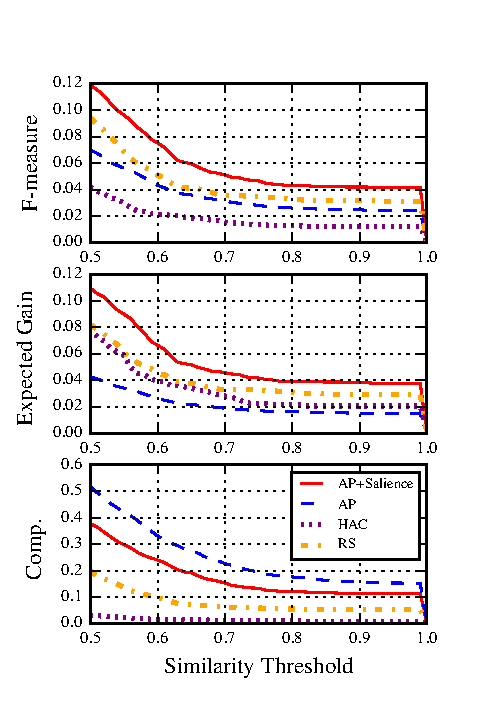
\includegraphics[]{chapter3/figures/nuggets-metrics2.eps}
\caption{Expected Gain and Comprehensiveness performance.}
\label{fig:3_aps_autots}
\end{wrapfigure}


\subsection{Model 2: LOLS}

Our next model attempts to address some of the shortcomings of the 
first. First the previous model process sentences in hourly batches.
Ideally we would process new documents as soon as possible in order 
to minimize the negative effects of latency. Second, our salience
regressors were statically trained and did not take advantage of features
like the similarity to recently selected updates and relied mostly on
tuned thresholds to account for redundancy. 

Getting around these limitations poses some severe challenges. Using
dynamic features means that naive traing will require gold reference
sentence extracts and that naively training a sentence salience model
with these will under explore the space of plausable update summaries,
meaning that in practice errors are likely to snowball over time.

Instead, we develop a clairvoyant oracle summarizer $\pi^o$ whose behavior
we want to imitate. $\pi^o$ has knowledge of what nuggets, if any, 
are present in each sentence in the document stream, and it's behavior
is quite simple: it processes each sentence in a query's relevant document 
stream and 
when it encounters a sentence with a novel nugget, it adds that sentence
to the update summary.

As we stated before, training only on a single oracle run over document stream
would be sub-optimal because the oracle is perfect and it would finish 
recovering all of the nuggets quite quickly and then do nothing for
the remainder of the stream. In practice, our learned model is likely to
make mistakes, missing the first few appearances of a nugget but hopefully
recovering them as repetition in the stream makes them more likely to be 
selected. Only following the oracle's first best pass would not help us learn
to recover from errors.

To make better use of the oracle, we adopt the locally optimal learning to
search (LOLS) algorithm \cite{lols}, one of a family of learning to search 
(L2S) algorithms. In order to formally describe the algorithm, we first 
introduce some notation. We treat the streaming summarization problem
as a markov decision process. At each timestep $t$ we observe a state
$s_t \in \mathcal{S}$ and $t$-th sentence $x_t \in \mathcal{X}$ from the 
document stream.
A policy $\pi : \mathcal{S} \times \mathcal{X} \rightarrow \{0, 1\}$
maps a state-sentence tuple to an action $a \in \mathcal{A} =\{0,1\}$
where $a=1$ indicates we extract the sentence and $a=0$ indicates we skip
the current sentence. The transition function 
$d : \mathcal{S} \times \mathcal{X} \times \mathcal{A} \rightarrow \mathcal{S}$
deterministically maps state-sentence-action tuples to the next state. 
In practice the state contains set of sentences previously extracted and
other rolling statistics from previously observed sentences in the stream.
Our training objective is to minimize the expected costs of each action:
\[ \mathcal{L}(\pi) = \mathbb{E}_{s,x \sim \pi} \left[ c\left(\pi(s,x), s, x\right) \right] \]
where $c :\mathcal{A} \times \mathcal{S} \times \mathcal{X} \rightarrow \mathcal{A}$ is the cost of taking a given action in a particular state-sentence
observation.

~\\

~\\

In the LOLS training regime, there are two phases: the 
\emph{roll-in} and the \emph{roll-out}. The roll-in phase 

at each timestep 
we alternate between using the oracle $pi^o$ or our current learned policy
$\hat{\pi}$ to run multiple time steps into the future and get a cost for 
a hypothetical summary we would have created in the case where we extracted the 
current sentence or skipped it. We collect these scores for each decision
and update a regression model to accuractely predict the cost of each action
given the current sentence and update summary/stream state.





\subsubsection{Data}
We ran 

\subsubsection{Oracle Policy and Loss Function}

We use a greedy oracle that selects sentences that contain novel
nuggets. This oracle will achieve an optimal Comprehensiveness score, i.e.
it will obtain every possible novel nugget in the roll-out phase.
However, it will not always achieve the maximum possible Expected Gain.
For example, consider the sequence of sentences $s_1, s_2, s_3$, where
nugget $n_1 \in s_1$, $n_2 \in s_2$, and $n_1,n_2 \in s_3$. The greedy oracle,
proceeding sequentially would select sentences $s_1$ and $s_2$, and skip
$s_3$, achieving an Expected Gain of $\frac{|\{n_1, n_2\}|}{|\{s_1, s_2 \}|} = \frac{2}{2} = 1$. The maximum achievable Expected Gain is obtained by skipping
the first two sentences and selecting sentence $s_3$ yielding $\frac{|\{n_1, n_2\}|}{|\{s_3 \}|} = \frac{2}{1} = 2$. In practice we are far from matching
the greedy oracle and so it suffices for now as an aspirational target.



We used the complement of Dice coefficient as the loss function.



\subsubsection{Experiments }

In our results, we refer to our learn-to-search approach as LS.
We compare to a lead sentence baseline that takes the first sentence
of every document as an update if it's maximum cosine similarity to any 
previous update was below a threshold. We refer to this method as COS.

We also compare our 








suboptimal in that it will achieve a perfect
Comprehensiveness 























